% Name: Function with asymptotes
% Description: The rational function x^2/(x^2 - 4), its three branches, and its vertical asymptotes x = -2 and x = 2 and horizontal asymptote y = 1 drawn dashed.
% Tags: asymptote, rational function, vertical asymptote, horizontal asymptote

\usepackage{pgfplots}
\pgfplotsset{compat=1.18}

\begin{tikzpicture}[asymptote/.style={dashed, gray!70!black, thick}]
  \begin{axis}[
    width=9cm, height=6.5cm, axis lines=middle, xlabel=$x$, ylabel=$y$,
    xmin=-6, xmax=6, ymin=-5, ymax=6, xtick={-4,4}, ytick={-4,-2,2,4},
    every axis plot/.append style={very thick, blue!70!black, samples=100},
  ]
    \addplot[domain=-6:-2.03] {x^2/(x^2 - 4)};
    \addplot[domain=-1.94:1.94] {x^2/(x^2 - 4)};
    \addplot[domain=2.03:6] {x^2/(x^2 - 4)};
    \draw[asymptote] (axis cs:-2,-5) -- (axis cs:-2,6) node[pos=0.73, right, font=\small] {$x = -2$};
    \draw[asymptote] (axis cs:2,-5) -- (axis cs:2,6) node[pos=0.73, left, font=\small] {$x = 2$};
    \draw[asymptote] (axis cs:-6,1) -- (axis cs:6,1) node[pos=0.02, below right, font=\small] {$y = 1$};
    \node[blue!70!black, font=\small, fill=white, inner sep=1pt] at (axis cs:4.1,3.6) {$y = \dfrac{x^2}{x^2 - 4}$};
  \end{axis}
\end{tikzpicture}
